% This is samplepaper.tex, a sample chapter demonstrating the
% LLNCS macro package for Springer Computer Science proceedings;
% Version 2.20 of 2017/10/04
%
\documentclass[runningheads]{llncs}
%
\usepackage{graphicx}
\usepackage{hyperref}
\usepackage{academicons}
\usepackage{xcolor}
\usepackage{multirow}
% Used for displaying a sample figure. If possible, figure files should
% be included in EPS format.
%
% If you use the hyperref package, please uncomment the following line
% to display URLs in blue roman font according to Springer's eBook style:
\renewcommand\UrlFont{\color{blue}\rmfamily}
\newcommand{\orcid}[1]{\href{https://orcid.org/#1}{\textcolor[HTML]{A6CE39}{\aiOrcid}}}


\begin{document}
%
\title{Forecasting security alerts based on time series}
% \title{Forecasting security alerts based on time series\thanks{Supported by organization x.}}
%\titlerunning{Abbreviated paper title}
% If the paper title is too long for the running head, you can set
% an abbreviated paper title here
%
\author{Patrik Pekar\v{c}\'{i}k\inst{1}\orcid{0000-0002-8818-0960} \and
Andrej Gajdo\v{s}\inst{2}\orcid{0000-0002-7004-6616} \and
Pavol Sokol\inst{3}\orcid{0000-0002-1967-8802}}
%
\authorrunning{P. Pekar\v{c}\'{i}k et al.}
% First names are abbreviated in the running head.
% If there are more than two authors, 'et al.' is used.
%
\institute{Pavol Jozef \v{S}af\'{a}rik University in Ko\v{s}ice, Faculty of Science, Ko\v{s}ice, Slovakia \email{patrik.pekarcik@upjs.sk} \and
Pavol Jozef \v{S}af\'{a}rik University in Ko\v{s}ice, Faculty of Science, Ko\v{s}ice, Slovakia \email{andrej.gajdos@upjs.sk} \and
Pavol Jozef \v{S}af\'{a}rik University in Ko\v{s}ice, Faculty of Science, Ko\v{s}ice, Slovakia \email{pavol.sokol@upjs.sk} }
%
\maketitle              % typeset the header of the contribution
%
\begin{abstract}
As the number of devices and users connected to the Internet increases, also the number of security threats and incident increases and reactive measures are not sufficient. For this reason, the emphasis is shifting to preventive measures. The forecast of an increase or decrease in the number of security attacks or incidents in the network of an organization can be very helpful in prevention measures. In this paper, we focus on the network security situation forecasting based on time series analysis. The main objective of this paper is to determine the effect of seasonality and sliding window on network security situation forecasting, and criteria for choosing the suitable time series. Our evaluation shows that the seasonality does not play an important role in time series analysis. Also, time series analysis methods with the usage of sliding windows have comparable forecasting results. The combination of Arima and Exponential smoothing methods (ETS), which achieved the best results within the research evaluation, proves to be a suitable candidate for the real-time forecasting model. 

\keywords{Cybersecurity \and Network security \and Situation awareness \and Forecasting \and Time series .}

\end{abstract}
%

\section{Introduction}
% introduction / motivation

The number of cyber threats and attacks targeted towards all varieties of~devices increases daily. The main topics in the field of cybersecurity are the detection of security incidents and the response to them. Security threats cannot be completely eliminated. Therefore, the current trend is to move from reactive to proactive activities~\cite{cho2020toward}. The main goal is to prevent or mitigate security incidents before they cause harm to the organization. 

% motivation / specific problem
Methods of predictive analysis play a significant role in predicting specific security incidents, predicting the next steps of the attacker or in predicting the security situation of the organization~\cite{Husak2018survey}. In this regard, we recognize three main approaches to predictive methods in cybersecurity:
\begin {itemize}
 \item attack projection, problem being predicting the next move of an adversary in a running attack by projecting the series of actions the attacker performs~\cite{Yang2014};
 \item attack prediction, problem being what type of attacks are going to happen where and when~\cite{Abdlhamed2017};
 \item security situation forecast, problem being forecast number of attacks or vulnerabilities in the network of the organisation~\cite{Leau2015}.
\end {itemize}

In this paper, we focus on the network security situation forecasting. It is based on general definition of the situational awareness: \emph{``Perception of the elements in the environment within a volume of time and space, the comprehension of their meaning and the projection of their status in near future''}~\cite{Endsley1988}. Therefore, the network security situation forecasting is a monitoring of cyber systems, understanding of the cybersecurity situation represented by modeling of cyber threats or relating security alerts and predicting the changes in cyber security situation~\cite{Husak2018survey}.  

There are a number of important issues that need to be addressed in this approach. The main problems are space and time requirements of the predictive methods, prediction window, criteria for suitable time series etc. % rozpísať

% research questions
To summarize the problems outlined above, we emphasize the following questions that we aim to answer:
\begin {enumerate}
 \item the effect of seasonality on network security situation forecasting,
 \item the effect of the sliding window on network security situation forecasting,
 \item time series selection criteria suitable for network security situation forecasting.
\end{enumerate}

% approach
To answer the questions, we use predictive methods based on time series. Time series models “attempt to make use of the time-dependent structure present in a set of observations”~\cite{condon2008analysis}. The appropriate forecasting methods depend largely on what type of data is available. We have the choice of either qualitative forecasting methods (in cases when available data are not relevant to the forecasts) or quantitative forecasting methods. For purpose of research in this paper, we have available data from Warden system~\cite{kacha2015warden} and we have chosen quantitative forecasting methods, which describe the network security situation at a point in time~\cite{Leau2015}.

This paper is based on the results of our previous research~\cite{Sokol2018}. In previous papers, we focused on the quantitative analysis of the total number of incidents and did not pay attention to different categories of alerts. In research paper~\cite{new_paper}, we address similar issues, but only work with weekly data. This paper clarifies the issues examined and uses annual data as source data, which, in addition to the quantitative component (number), also carry a qualitative component (alert category, network protocol, or network port).

% paper structure
This paper is organized into five sections. Section 2 focuses on  the review of published research related to predictions in cybersecurity based on time series. Section 3 focuses on the research methodology and outlines the dataset and methods used for the analysis. Section 4 states result from an analysis of the research questions and discuss knowledge obtained from the analysis. The last section contains conclusions.

\section{Related works}

% intro
This section provides an overview of papers that focus on the prediction of security attacks, security incidents or security threats using time series analysis. Most of the papers focus on the detection of attacks rather than a prediction of attacks~\cite{liu2015cloudy}. Papers~\cite{condon2008analysis} and~\cite{werner2017time}. Authors in~\cite{werner2017time}  aim to exploit temporal correlations between the number of attacks per day in order to predict the future intensity of cyber incidents. On the other hand,~\cite{wei2012intrusion} focuses on the prediction of attack based on ARMA time series model. In the paper, authors focused on modelling and analyzing traffic flow data by time-sequence techniques. Also, they proposed a data traffic prediction model based on the autoregressive moving average (ARMA) using the time series data.

%focus on prediction of security incident based on ARIMA time series model. In~\cite{condon2008analysis}, authors discuss time series models with a broad set of security incident data. They also compare the forecasts from time series models with forecasts from Non-Homogeneous Poisson Process (NHPP) software reliability growth (SRG) models. Another paper focused on prediction of attack based on ARIMA time series is~\cite{werner2017time}. It aims to exploit temporal correlations between the number of attacks per day in order to predict the future intensity of cyber incidents. They were interested in 4 types of attacks - denial of service (DOS), malicious email, malicious URL, and attack on internet-facing service.

%It proposes an intrusion detection system for wireless networks for industrial automation-process automation (WIA-PA). 


Another research groups conduct research in the field of prediction of attack based on generalized ARCH (GARCH) models. In~\cite{tang2016exploiting}, authors propose a framework for statistically analyzing long-term vulnerability time series between January 1999 and January 2016. For this purpose, generalized ARCH (GARCH) models and SARIMA model are used for the National Vulnerability Database. Another example is~\cite{zhan2015predicting}. Authors use grey-box FARIMA+GARCH models and discuss the integration of Extreme Value Theory (EVT) and the Time Series Theory (TST). In this paper, they show that EVT can offer long-term predictions (e.g. 24-hour ahead-of-time), while gray-box TST models can predict attack rates 1-hour ahead-of-time at an accuracy that can be deemed practical.

In the field of prediction of attacks, it is necessary to mention also paper~\cite{soldo2011blacklisting}. Authors focus on the problem of forecasting attack sources based on past attack logs from several contributors. They evaluate and combine several factors - attacker-victim history using time-series, attackers and/or victims interactions using neighbourhood models and global patterns using singular value decomposition. In terms of time series analysis, they use an Exponential Weighted Moving Average (EWMA) model.

\section{Methodology}

\subsection{Dataset}
The source of data for our research is the alerts obtained from a Warden system~\cite{kacha2015warden}. It is a system that supports sharing information about security events on individual computer networks connected to this system. Data is stored and shared in IDEA (Intrusion Detection Extensible Alert) format~\cite{kacha2014idea}. IDEA format is a descriptive data model using a key-value JSON structure.

The main detection sources of data that send IDEA alerts to the Warden system can include attack detection systems, honeypots, network flow probes, system log records, and other data sources deployed in several networks (Czech national research and education network, Czech commercial network). Alert in the IDEA format contains several mandatory fields (format, ID, detect time, category)~\cite{kacha2014idea} and many optional fields with multiple input support. The fields we follow most in this research are the category, network traffic source data (IP address, port, protocol), network traffic target data (IP, port, protocol), detection time, and interruption time. For this research, data were collected during one year (from 2017-12-11 to 2018-12-11) by the Warden system. Collected data contain approximately one billion records from various data sources mentioned above. 

For purposes of this research, we processed one-year dataset to 21 time series based on different criteria. Criteria were chosen from all possible values of category, port and protocol fields by statistical representation throughout the whole dataset. The criterion has to meet the requirement occurrence of the value in at least 1\,\% alerts of all alerts. Chosen criteria are followings: (I) Count of all alerts; (II) Count of unique IP; (III) Category recon scanning; (IV) Category availability DDoS; (V) Category attempt login; (VI) Category attempt exploit; (VII) Category malware ransomware; (VIII) Category intrusion botnet; (IX) Port 21; (X) Port 22; (XI) Port 23; (XII) Port 25; (XIII) Port 80; (XIV) Port 443; (XV) Port 445; (XVI) Protocol TCP; (XVII) Protocol SSH; (XVIII) Protocol UDP; (XIX) Protocol ICMP; (XX) Protocol Microsoft WBT Server; (XXI) Protocol telnet. Furthermore these time series was processed to multiple version based on reference time period. We have made time series with 1 minute, 10 minutes, 15 minutes, 30 minutes and 60 minutes time period.ime series is stored in PostgreSQL database with TimescaleDB extension. TimescaleDB extension is important for our future aggregations to create different views on created time series data.

%\textcolor{green}{IDEA alerts was stored in number of SQLite databases sized about 100 GB each. This databases contained approximately 40 - 50 days of collected data. During analysis of data we found out that SQLite storage has changed order of received data. With this resolution we decided to split SQLite files per days. This split made 365 SQLite databases sized about 1-2 GB. After this preprocessing of nearly 3/4 of TB we was able to stream all IDEA alerts in same order as we collected them. IDEA alerts was then streamed to real-time python scripts. Role of this scripts was calculation sum for different criteria mentioned above during period of one-minute. Calculated sums was then saved to PostgreSQL database with TimescaleDB extension. TimescaleDB extension is important for our future aggregations to create different views on created time series data.}


\subsection{Method Description}

There is a wide range of quantitative forecasting methods and their usage often depends on the specific disciplines, on the  nature of data or specific purposes. For choosing a particular method, properties, accuracies, and computational costs must be considered. In our research, we have considered four approaches to time series forecasting: (I) ARIMA models; (II) Exponential smoothing models (state space models); (III) the naive approach; and (IV) combination (average) of ARIMA and Exponential smoothing models.

The most commonly used classes of models in time series modelling and forecasting are ARIMA and Exponential smoothing (ETS)~\cite{hyndman2018forecasting}. We compared them with the naive methods~\cite{brockwell2016introduction,box2015time}, which can process large data sets and they do not have high computational requirements. They serve as a benchmark for predictions in our research. We also added a combination (average) of the ARIMA and ETS methods to compare the standard methods with their combination. The idea  of averaging or boosting is very popular in machine learning nowadays~\cite{Husak2018survey}. 

Prediction using ETS family models is characterized by a weighted combination of older observations with new ones. The new observations have a relatively higher weight compared to the older observations. Exponential smoothing reflects the fact that weights decrease exponentially as observations age~\cite{hyndman2018forecasting,brockwell2016introduction}.

The ARIMA models represent a generalization of the class of ARMA models that incorporate a wide range of non-stationary series. These models, by finite number of differentiations, ensure time series stationarity, allowing the use of ARMA models. ARMA models are a combination of auto-regression (AR) and moving average (MA)~\cite{box2015time}. The ETS class provides another approach to time series modelling and forecasting. While ETS models are based on a description of the trend and seasonality in the data, ARIMA models aim to describe the autocorrelations in the data~\cite{hyndman2018forecasting}. Both classes of models can reflect seasonality in the data. 

%ARIMA model can be expressed by the formula:
% 
%\begin{equation}
%y_t^{(d)} = c + \sum_{i = 1} ^ {p} \phi_{i} y_{ti}^{(d)} + \sum_{j = %1}^{q} \theta_j \varepsilon_{tj} + \varepsilon_t
%\end{equation}
% 
%where $y$ is the series differentiated $d$ times, $c$ is the %constant, $p$ is the degree of autoregression, $\phi_i$ are the %coefficients of autoregression, $q$ is the degree of moving averages, $\theta_J$ are the coefficients of moving averages and $\varepsilon_t$ are errors.


\subsection{Experiment evaluation}
The research questions were evaluated using above mentioned dataset from the Warden system. We evaluated the methods using the implementation presented in our previous work~\cite{Sokol2018,new_paper}. In our extensive calculations, we used R functions from one of the most common R-packages for time series predictions called \textit{forecast}~\cite{hyndman2007automatic}. Beneficial features when working with large data sets or potentially in real-time prediction are those used to automatically fit ARIMA or ETS. These functions are designed to automatically select the best model from the considered class under given conditions, for example, taking into account information criteria~\cite{hyndman2007automatic}.

%\textcolor{blue}{All the above-mentioned types of models were evaluated and compared according to several criteria based on the quality of predictions. poznamka TM- tato veta sa v clanku opakuje niekolko krat, uz na tomto miesta nedava nave info} 
For each class of models, particular models were fitted in the seasonal and non-seasonal settings. Seasonal variation, or seasonality means cycles that repeat regularly over time. A cycle structure in a time series may or may not be seasonal. If it consistently repeats at the same frequency, it is seasonal, otherwise it is not seasonal and is called a cycle. We considered one, two, five, and ten steps ahead predictions, which were compared to true values included in the test set. 

Furthermore, we considered two cases of model fitting. The first one was the “classical” one; when we kept the whole training dataset and step by step, we added one more observations from the test set to training set in each round of evaluation. In the second case, we used the so-called “rolling window” or “one in, one out”, which means that in each round of evaluation we remove the oldest observation from the training set and at the same time we add one new observation from the test set to training set.

At first, we calculated 95\,\% (bootstrap) prediction intervals, and consequently, the average coverage was computed. It is the percentage of all confidence intervals which covered the true (future) value of particular time series. It should be close to 95\,\%. The values approaching 95\,\% indicate that the 95\,\% prediction interval works well for a specific case (method, number of forecast steps and time interval). If the coverage is lower than 95\,\%), it points out the lower reliability of prediction interval. Conversely, the higher the coverage (more than 95\,\%) the wider and less informative prediction interval.

We also took a look at the average length of prediction intervals. In general, shorter prediction intervals are considered more precise (under the fixed confidence level). They give us better information about the future values of time series. We have divided our evaluation into two stages. In the first stage We evaluated forecasting methods only on the total number of alerts and did not address the qualitative component (alert category, network protocol, or network port). In previous work~\cite{new_paper} we considered 24 hours period and four different time units (5 minutes, 15 minutes, 30 minutes and 60 minutes) considering the  fact that dataset usage in this work consists of data for one week. In this paper, we extend our evaluation. Given the fact that we use one-year dataset and based on results from previous work, we considered 24 hours and 7 days period with two different time units (30 minutes and 60 minutes), and two different lengths of datasets (month, two months). We decided to choose the last two months from the entire one year dataset because of the time complexity in our extensive numerical study. Moreover one can assume that time series values far in the past (with respect to time units) would not have a significant impact on predictions of future values. Main aim of this stage is to answer the issues of seasonality and the usage of rolling windows in the perspective of long-term period (one year). 

In the second stage of our evaluation, we used the best combination of time interval, period, and forecasting period (30 minutes, 7 days, one month). In this stage, we evaluated forecasting methods on 21 attributes of alerts and we address the qualitative component (alert category, network protocol, or network port). Main aims of this stage was to analyse seasonality and the usage of rolling-windows in other time series taking into account qualitative component. Also, we analysed criteria for time series suitable for forecasting.     

\section{Results and discussion}

In this section, we describe in more detail both stages of experiment evaluation. We take a closer look at the individual results and discuss research questions based on them.

%-------------------------------------------------------
% The first stage - results
%-------------------------------------------------------
\subsubsection{Results of the second stage of  evaluation}

As a part of evaluation, in the first stage we tested all above mentioned methods in six cases (time interval, time period, time unit): (I) 30 minutes, 24 hours, 1 month; (II) 30 minutes, 7 days, 1 month; (III) 60 minutes, 24 hours, 2 months; (IV) 60 minutes, 24 hours, 1 month; (V) 60 minutes, 7 days, 2 months; (VI) 60 minutes, 7 days, 1 month.


% ------------- cross-validation  -----------------------------

The first approach to evaluate the predictions’ quality of particular models is the so-called cross-validation~\cite{hyndman2018forecasting}. We employed two variations of this approach. In the first case, we calculated the predictions at specific future times (separately for one or two or five or ten steps ahead) throughout the test set, and at the end we calculated the metric value from all the predictions for the various prediction steps separately. The metric commonly used to evaluate forecast accuracy is the mean absolute error rate (MASE)~\cite{hyndman2006another}. 
It is a prefered metric as it is less sensitive to outliers, more easily interpreted and less variable on small samples. 
MASE is defined as~\cite{hyndman2018forecasting}:

% 
\begin{equation}
\textrm{MASE} = \textrm{mean}(|q_j|)
\end{equation}
% 
where, for non-seasonal time series, $q_j$ is:
% 
\begin{equation} 
q_j= \frac{e_j}{\frac{1}{T-1} \sum_{i=2}^{T}|y_i - y_{i-1}|},
\end{equation}
% 
and, for seasonal time series, $q_j$ is:
% 
\begin{equation} 
q_j = \frac{e_j}{\frac{1}{T-m} \sum_{i=m+1}^{T}|y_i - y_{i-m}|}
\end{equation}

In both cases, $e_j$ is forecast error, i.e., the difference between an observed value and its forecast, $y_j$ represents observed value, $T$ is the length of time series, and $m$ is seasonality parameter (period).

In the second type of cross-validation, we considered all forecasts  up to the second, fifth and tenth step ahead forecast in each round of evaluation we calculate MASE (not just the last one as in the previous case). According to this criterion, the prediction is more accurate, when the lower value (ideally below 1) of MASE is achieved. A scaled error is less than one if it arises from a better forecast than the average naive forecast computed on the training data. Conversely, it is greater than one if the forecast is worse than the average naive forecast computed on the training data~\cite{hyndman2014measuring}.

\begin{table}[h]
    \centering
    \begin{tabular}{c|c|c|c|c|c|c} \hline
        Case & \,30/24/1\, & \,30/7/1\, & \,60/24/2\, & \,60/24/1\, & \,60/7/2\, & \,60/7/1\, \\    
        \hline\hline
       \multirow{2}{*}{Two-steps} & 0.4755 & 0.4009 & 0.7159 & 1.1612 & 0.5598 & 0.9888 \\
       & AEsw,AEw & AEsw,AEw & AEsw,AEw & AEsw,AEw & AEsw,AEw & AEsw,AEw  \\
        \hline
        \multirow{2}{*}{Five-steps} & 0.5539 & 0.4674 & 0.765 & 1.2023 & 0.5978 & 1.0249 \\
        & AEsw,AEw & AEsw,AEw & AEsw,AEw & AEsw,AEw & AEsw,AEw & AEsw,AEw  \\
        \hline
        \multirow{2}{*}{Ten-steps} & 0.6331 & 0.5369 & 0.8038 & 1.2239 & 0.6281 & 1.0453 \\
        & AEsw,AEw & AEsw,AEw & AEsw,AEw & AEsw,AEw & AEsw,AEw & AEsw,AEw  \\
        \hline     
    \end{tabular}
    \caption{Results of the average MASE values for forecasting methods. Notes: A - ARIMA model; E - Exponential Smoothing (state space models); N - naive model; AE - ARIMA + Exponential smoothing (average); s - with seasonality; (s) - with seasonality for each model in cell; w - rolling window.}
    \label{tab:mase}
\end{table}

Table~\ref{tab:mase} shows the results of the average MASE values for 2-step forecasts, 5-step forecasts, and 10-step forecasts calculated over the whole training set. Except one case (60 minutes, 7 days, 2 months), all values were below 1. Overall, the best method seems to be the combination (average) of ARIMA and Exponential smoothing models with a sliding window. In the case of the second type of cross-validation (average MASE values), this method has the best results in all monitored cases. The ETS method appears to be a suitable method at 60-minutes intervals. In contrast, at 30-minutes, the ARIMA method has the best results for 5-steps and 10-steps forecasts. 

% ------------- prediction interval  -----------------------------

The second approach to assessing the quality of predictions of specific models is an average coverage of 95\,\% by prediction intervals. We used the above six cases and compared the established forecasting approaches based on different prediction steps - next, second, 5th and 10th step ahead. 

\begin{table}[h]
    \centering
    \begin{tabular}{c|c|c|c|c|c|c} \hline
        Case & \,30/24/1\, & \,30/7/1\, & \,60/24/2\, & \,60/24/1\, & \,60/7/2\, & \,60/7/1\, \\
     \hline\hline
        \multirow{2}{*}{One-step} & 96.6667 & 96.6667 & 94.0625 & 88.125 & 94.0625 & 88.125 \\
        & Es,E,Ar & AEs,Esr,A,Er & Asr,AEsr & Ns,Nsr,Nr & Er,AEr & Ns,Nsr,Nr  \\
        \hline
        \multirow{2}{*}{Two-steps} & 95.8194 & 95.8194 & 94.2006 & 87.4214 & 94.0439 & 87.4214 \\
        & Es,E & AEs,Esr,A,Er & AEsr & Nr & Er & Nr \\
        \hline
        \multirow{2}{*}{Five-steps} & 95.1351 & 95.0676 & 95.1266 & 89.7436 & 95.1266 & 89.7436 \\
        & E & Er & Nsr,Nr & Nsr,Nr & Nsr,Nr & Nsr,Nr  \\
        \hline
        \multirow{2}{*}{Ten-steps} & 95.2234 & 95.189 & 94.5016 & 94.9007 & 94.5016 & 94.9007 \\
        & A & A &	AEsr & Ns,Nr & Er & Ns,Nr \\
        \hline
    \end{tabular}
    \caption{Average percentage coverage of actual (future) time series values by 95\,\% prediction intervals. Notes: A - ARIMA model; E - Exponential Smoothing (state space models); N - naive model; AE - ARIMA + Exponential smoothing (average); ALL - all models; (-) - without; s - with seasonality; w - rolling window.}
    \label{tab:avg_95}
\end{table}

The table~\ref{tab:avg_95} shows the results of the average coverage of 95\,\% prediction intervals. The values of average coverage in two cases with time unit of 30 minutes (monthly data) and in  two cases with time unit of 60 minutes (bimonthly data) are close to nominal value 95 and these predictions intervals are not too wide. It implies they are quite precise. Vice versa, values of the average coverage in two cases with 60 minutes time intervals and bimonthly data are below the nominal value 95 so these prediction intervals are not very reliable or they can be considered as biased.

The main aim of the first stage of  experimental evaluation was to determine an  appropriate case. According to results mentioned above the most suitable scenario for the methodology chosen by us is the case with monthly data, time intervals of 30 minutes, period equal to 7 days. The suitability of the selection of the 7-day period is also confirmed by the research based on time-oriented analysis and visualization of data collected by honeypots~\cite{sokol2015study}. Data set with these parameters was consequently analyzed in more details in the second stage.  

%-------------------------------------------------------
% The second stage - results
%-------------------------------------------------------
\subsubsection{Results of the second stage of the evaluation}

In the second stage we tested all above mentioned methods with the best result case (30 minutes, 7 days, 1 month) on 16 selected time series. Six time series have been removed from the evaluation process due to fact, that they contained small counts (less than 100 -- e.g. category availability DDoS) or they contained mostly zeros (e.g. category malware -- ransomware). If the counts are large enough (more than 100) then the difference between a continuous sample space and the discrete sample space has no perceivable effect on the forecasts~\cite{hyndman2018forecasting}. However, if our data contains small counts (less than 100) then we need to use forecasting methods that are more appropriate for a sample space of non-negative integers. For instance the so called Croston's method can be considered~\cite{Croston1972ForecastingAS,Christou2015}. On the other hand the time series with mostly zeros can be suitable  for time series anomaly detection~\cite{mehrotra2017anomaly} and it is an interesting direction for future research.

\begin{table}[h]
    \centering
    \begin{tabular}{c|c|c|c|c|c|c|c|c} \hline
        \multirow{2}{*}{Time series} & Count & Recon & Attempt & Attempt & Intrusion & Port & Protocol & Protocol  \\
              &  & Scanning & Login & Exploit  & Botnet & 80 & SSH & Telnet  \\
        \hline\hline
        \multirow{3}{*}{Two-steps} & 0.397 & 0.449 & 0.1457 & 0.8304 & 0.1985 & 0.1764 & 0.1662 & 0.8983 \\
        & AEsw & AEsw & AEsw & AEsw & Aw & AEsw & AEsw & AEsw  \\
        & AEw & AEw & AEw & AEw &  & AEw & AEw & AEw \\
        \hline
        \multirow{3}{*}{Five-steps} & 0.4633 & 0.5151 & 0.2078 & 0.8271 & 0.2112 & 0.1868 & 0.2221 & 0.9726 \\
        & AEsw & AEsw & AEsw & AEsw & As & AEsw & AEsw & AEsw  \\
        & AEw & AEw & AEw & AEw & Asw, A & AEw & AEw & AEw \\
        \hline
        \multirow{3}{*}{Ten-steps} & 0.5335 & 0.5839 & 0.2595 & 0.8191 & 0.2133 & 0.1975 & 0.2697 & 0.9832 \\
        & AEsw & AEsw & AEsw & AEsw & As & AEsw & AEsw & AEsw  \\
        & AEw & AEw & AEw & AEw & Asw, A & AEw & AEw & AEw \\
        \hline     
    \end{tabular}
    \caption{Results of the average MASE values for forecasting methods. Notes: A - ARIMA model; E - Exponential Smoothing (state space models); N - naive model; AE - ARIMA + Exponential smoothing (average); s - with seasonality; (s) - with seasonality for each model in cell; w - rolling window.}
    \label{tab:mase_2nd_stage}
\end{table}


Table~\ref{tab:mase_2nd_stage} shows the results of the average MASE values for 2-step forecasts, 5-step forecasts and 10-step forecasts calculated for 16 time series. In this table the significant time series for discussion are showed. The results from the 2nd stage of research evaluation confirm the findings from the first stage. The best method seems to be the combination (average) of ARIMA and Exponential smoothing models. Although the methods with sliding window do not have the best results in all cases (16-time series), their results in the average MASE value are close to the best method.

Example of usage of forecasting method based on time series is shown in Figure~\ref{fig:forecast_attempt_login} and Figure~\ref{fig:forecast_attempt_exploit}, where we can see one-step forecasting based on the combination of ARIMA and ETS (30 minutes time unit) for attribute "category attempt login" (Figure~\ref{fig:forecast_attempt_login}) and for attribute "category attempt exploit" (Figure~\ref{fig:forecast_attempt_exploit}). These two categories of security alerts show the difference between time series based on security data, which we should consider. Both time series have a relatively sufficient number of data (Attempt login - 46.709.781 (7.74\,\% of the total number of alerts) and Attempt exploit - 27.695.575 (4.59\,\% of total alerts)). The difference lies in the nature of data. The second time series is hardly predictable~\cite{hendry1995dynamic} (you can see that predictions are far away from true values many times) because it looks like a white noise (random walk process). In such  situation it is difficult to find something reliable and better than naive forecasting methods due to the lack of correlation structure or some other patters which could be captured by sophisticated models. On the contrary the time series in Figure 1 shows some kind of structure and patterns and also the predictions are better compared to the previous case.  

\begin{figure}[h]
  \centering
  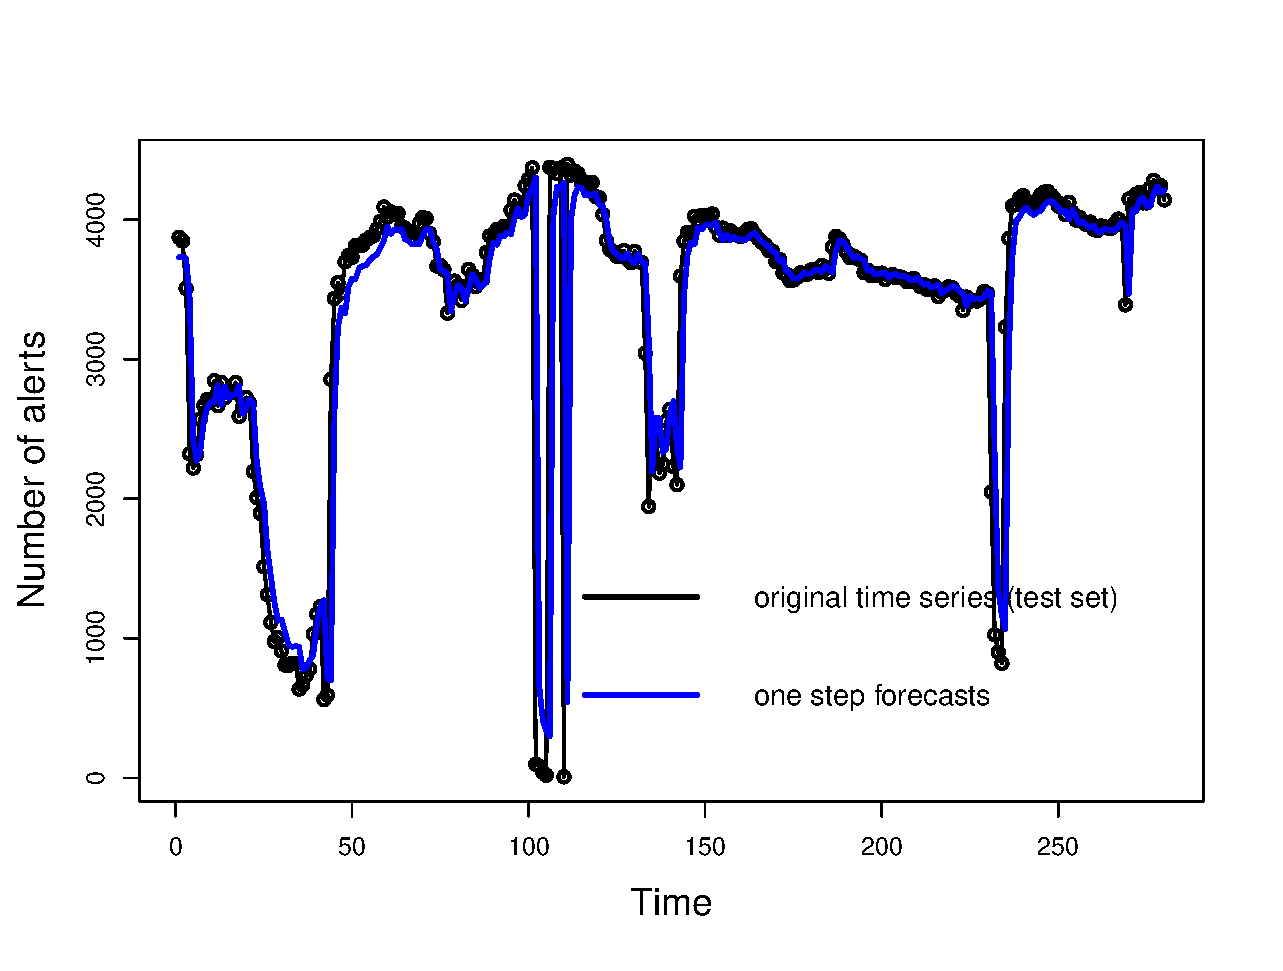
\includegraphics[width=0.7\textwidth]{images/item61_1step_forecasts_new.eps}
  \caption{One-step forecasting for attribute "category attempt login".} 
  \label{fig:forecast_attempt_login}
\end{figure}

\begin{figure}[h]
  \centering
  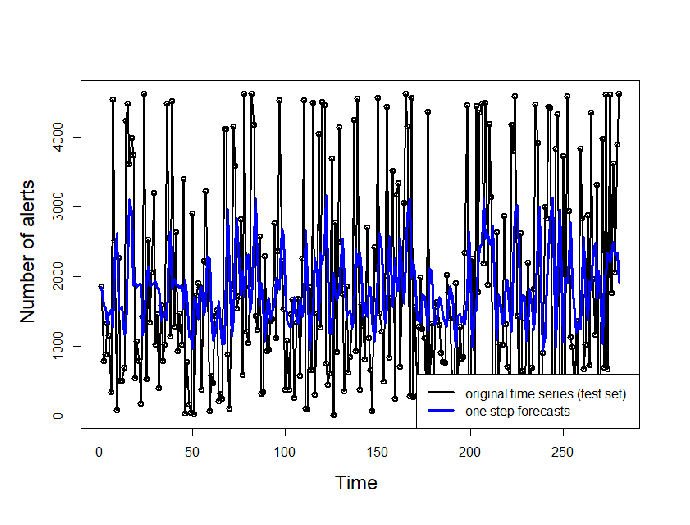
\includegraphics[width=0.7\textwidth]{images/item62_1step_forecasts_new.eps}
  \caption{One-step forecasting for attribute "category attempt exploit". }
  \label{fig:forecast_attempt_exploit}
\end{figure}


%-------------------------------------------------------
% Research questions - discussion
%-------------------------------------------------------

\subsubsection{Discussion of research questions}

% ------------- Seasonality  -----------------------------
As mentioned above, seasonal variation or seasonality means cycles that repeat regularly over time. We selected both ETS and ARIMA methods since they are able to reflect seasonality in the data. Our assumption is that seasonality does not need to be taken into account, as the patterns in  data (number of security alerts) do not repeat regularly (just irregularly in few cases) over time, but they depend on other factors. As the results show, the best values for individual forecasting are always achieved by the method in both its forms - taking into account, resp. disregarding seasonality. From this point of view, we can state that in time series based only on the total number of attacks, the seasonality does not play an important role in forecasting. 

% ------------- Rolling window  -----------------------------
As it can be seen from our results (table~\ref{tab:mase} and table~\ref{tab:avg_95}) the best performing forecasting approaches were those, which employed the so called rolling window technique. It is a good outcome because from the practical point of view it is not necessary to keep the whole dataset in memory and there is no need to fit models, make computations and predictions using the entire data set. It makes sense to find a reasonable window which is usually much shorter than the length of original data set. Again this can be an advantage when it comes to real-time predictions. In our numerical study we considered the length of window to be the 80\,\% of monthly data (time unit -- 30 min.) or 80\,\% of bimonthly data (time unit -- 60 min.). 

\section{Conclusion and future works}

As we mentioned in this paper several times, forecasting methods for this research were chosen so that they could find a suitable model themselves. The reason is the fact that the aim of the on-coming research is the real-time forecasting of security alerts. For this purpose, it is necessary to solve several issues,  e.g. issue of seasonality or the issue of the sliding window usage. In this paper, we focus on these issues and verify our assumptions using four methods and one-year dataset of security alerts. The results confirmed the assumption that seasonality is not necessarily taken into account, as well as the possibility of using a time window. These results are important for selecting an appropriate method for real-time processing. The combination of Arima and ETS methods, which achieved the best results within the research evaluation, proves to be a suitable candidate for the real-time forecasting model.
%Our future research will focus on the evaluation of the finding from this paper for real-time forecasting of security alerts.

\subsubsection*{Acknowledgment.}
This research is funded by the VVGS projects under contracts No. VVGS-PF-2020-1423 and No. VVGS-PF-2020-1427 and Slovak Research and development agency project under contract No. APVV-17-0561.

% ---- Bibliography ----
\bibliographystyle{splncs04}
\bibliography{bibliography.bib}

\end{document}
